	%!TEX program = xelatex
% 完整编译: xelatex -> bibtex -> xelatex -> xelatex
\documentclass[lang=cn,12pt,a4paper,cite=authoryear]{elegantpaper}

\title{统计学习实验三:Logistics Regression}
\author{王嗣萱 2018110601014}
\date{}


% 本文档命令
\usepackage{array}
\newcommand{\ccr}[1]{\makecell{{\color{#1}\rule{1cm}{1cm}}}}

\begin{document}

\maketitle

\section{实验原理}

\subsection{Logistic 分布}
Logistic 分布是一种连续型的概率分布,其分布函数和密度函数分别为:
\begin{equation}
	\begin{aligned}
		&F(x) = P(X \leq x)=\frac{1}{1+e^{-(x-\mu)/\gamma}} \\
		&f(x) = 	F^{'}(X \leq x)=\frac{e^{-(x-\mu)/\gamma}}{\gamma(1+e^{-(x-\mu)/\gamma})^{2}}
	\end{aligned}
\end{equation}

其中, $\mu$ 表示位置参数, $\gamma$ 为形状参数。我们可以看下其图像特征:

\begin{figure}[htbp]
	\centering
	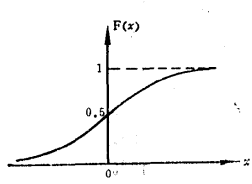
\includegraphics[width=0.3\textwidth]{lo_1.png}
	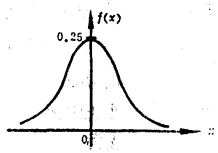
\includegraphics[width=0.3\textwidth]{lo_2.png}
	\caption{Logistic 分布}
\end{figure}

Logistic 分布是由其位置和尺度参数定义的连续分布。Logistic 分布的形状与正态分布的形状相似,但是 Logistic 分布的尾部更长,所以我们可以使用 Logistic 分布来建模比正态分布具有更长尾部和更高波峰的数据分布。在深度学习中常用到的 Sigmoid 函数就是 Logistic 的分布函数在  $\mu=0, \gamma=1$ 的特殊形式。

\subsection{Logistic 回归}
本次实验中考虑'0','1'的二分类问题,即一个伯努利分布。

Sigmoid函数,也称为逻辑函数(Logistic function):
\begin{equation}
	g(z)= \frac{1}{1+e^{-z}}
\end{equation}


逻辑回归的假设函数形式如下:
\begin{equation}
	\begin{aligned}
		&h_\theta(x) = g(\theta^T x), g(z)= \frac{1}{1+e^{-z}}
		\\
		&P(y=1|x;\theta)=h_{\theta}(x) 
		\\
		&P(y=0|x;\theta)=1-h_{\theta}(x)
	\end{aligned}
\end{equation}
可以将其合并为一个表达式:
\begin{equation}
	\begin{aligned}
		&P(y|x;\theta)=(h_{\theta}(x))^{y}(1-h_{\theta}(x))^{1-y}
	\end{aligned}
\end{equation}

logistic regression的目标函数是根据最大似然思想求得的。似然函数为:
\begin{equation}
	\begin{aligned}
		&L(\theta)=\prod_{i=1}^{n}(h_{\theta}(x^{i}))^{y^{i}}(1-h_{\theta}(x^{i}))^{1-y^{i}}
	\end{aligned}
\end{equation}


对$L(\theta)$求对数可以得到:
\begin{equation}
	\begin{aligned}
		&l(\theta)=-logL(\theta)=-\sum_{i=1}^{n}[{y^{i}}log(h_{\theta}(x^{i}))+(1-y^{i})log(1-h_{\theta}(x^{i}))]
	\end{aligned}
\end{equation}

使用$J(\theta)=\frac{1}{m}l(\theta)=-\frac{1}{N}logL(w) $作为logistic regression的损失函数



\subsection{}

\section{Python代码实现}

\section{结果及图形展示}

\section{总结体会}

\end{document}
